\chapter[Models]{Physical and numerical models}

\section{Physical and mathematical description} 

Characteristic of compositional multiphase models is that the phases
are not only matter of a single chemical substance. Instead, their
composition in general includes several species, and for the mass transfer, 
the component behavior is quite different from the phase behavior. In the following, we
give some basic definitions and assumptions that are required for the
formulation of the model concept below. As an example, we take a
three-phase three-component system water-NAPL-gas
\cite{A3:class:2002a}. The modification for other multicomponent
systems is straightforward and can be found, e.\ g., in
\cite{A3:bielinski:2006,A3:acosta:2006}.

\subsection{Basic Definitions and Assumptions for the Compositional
  Model Concept}
\textbf{Components:}
The term {\it component} stands for constituents of the phases which
can be associated with a unique chemical species, or, more generally, with 
a group of species exploiting similar physical behavior. In this work, we
assume a water-gas-NAPL system composed of the phases water (subscript
$\text{w}$), gas ($\text{g}$), and NAPL ($\text{n}$). These phases are
composed of the components water (superscript $\text{w}$), air
($\text{a}$), and the organic contaminant ($\text{c}$) (see Fig.\
\ref{A3:fig:mundwtrans}).
%
\begin{figure}[hbt]
  \centering
  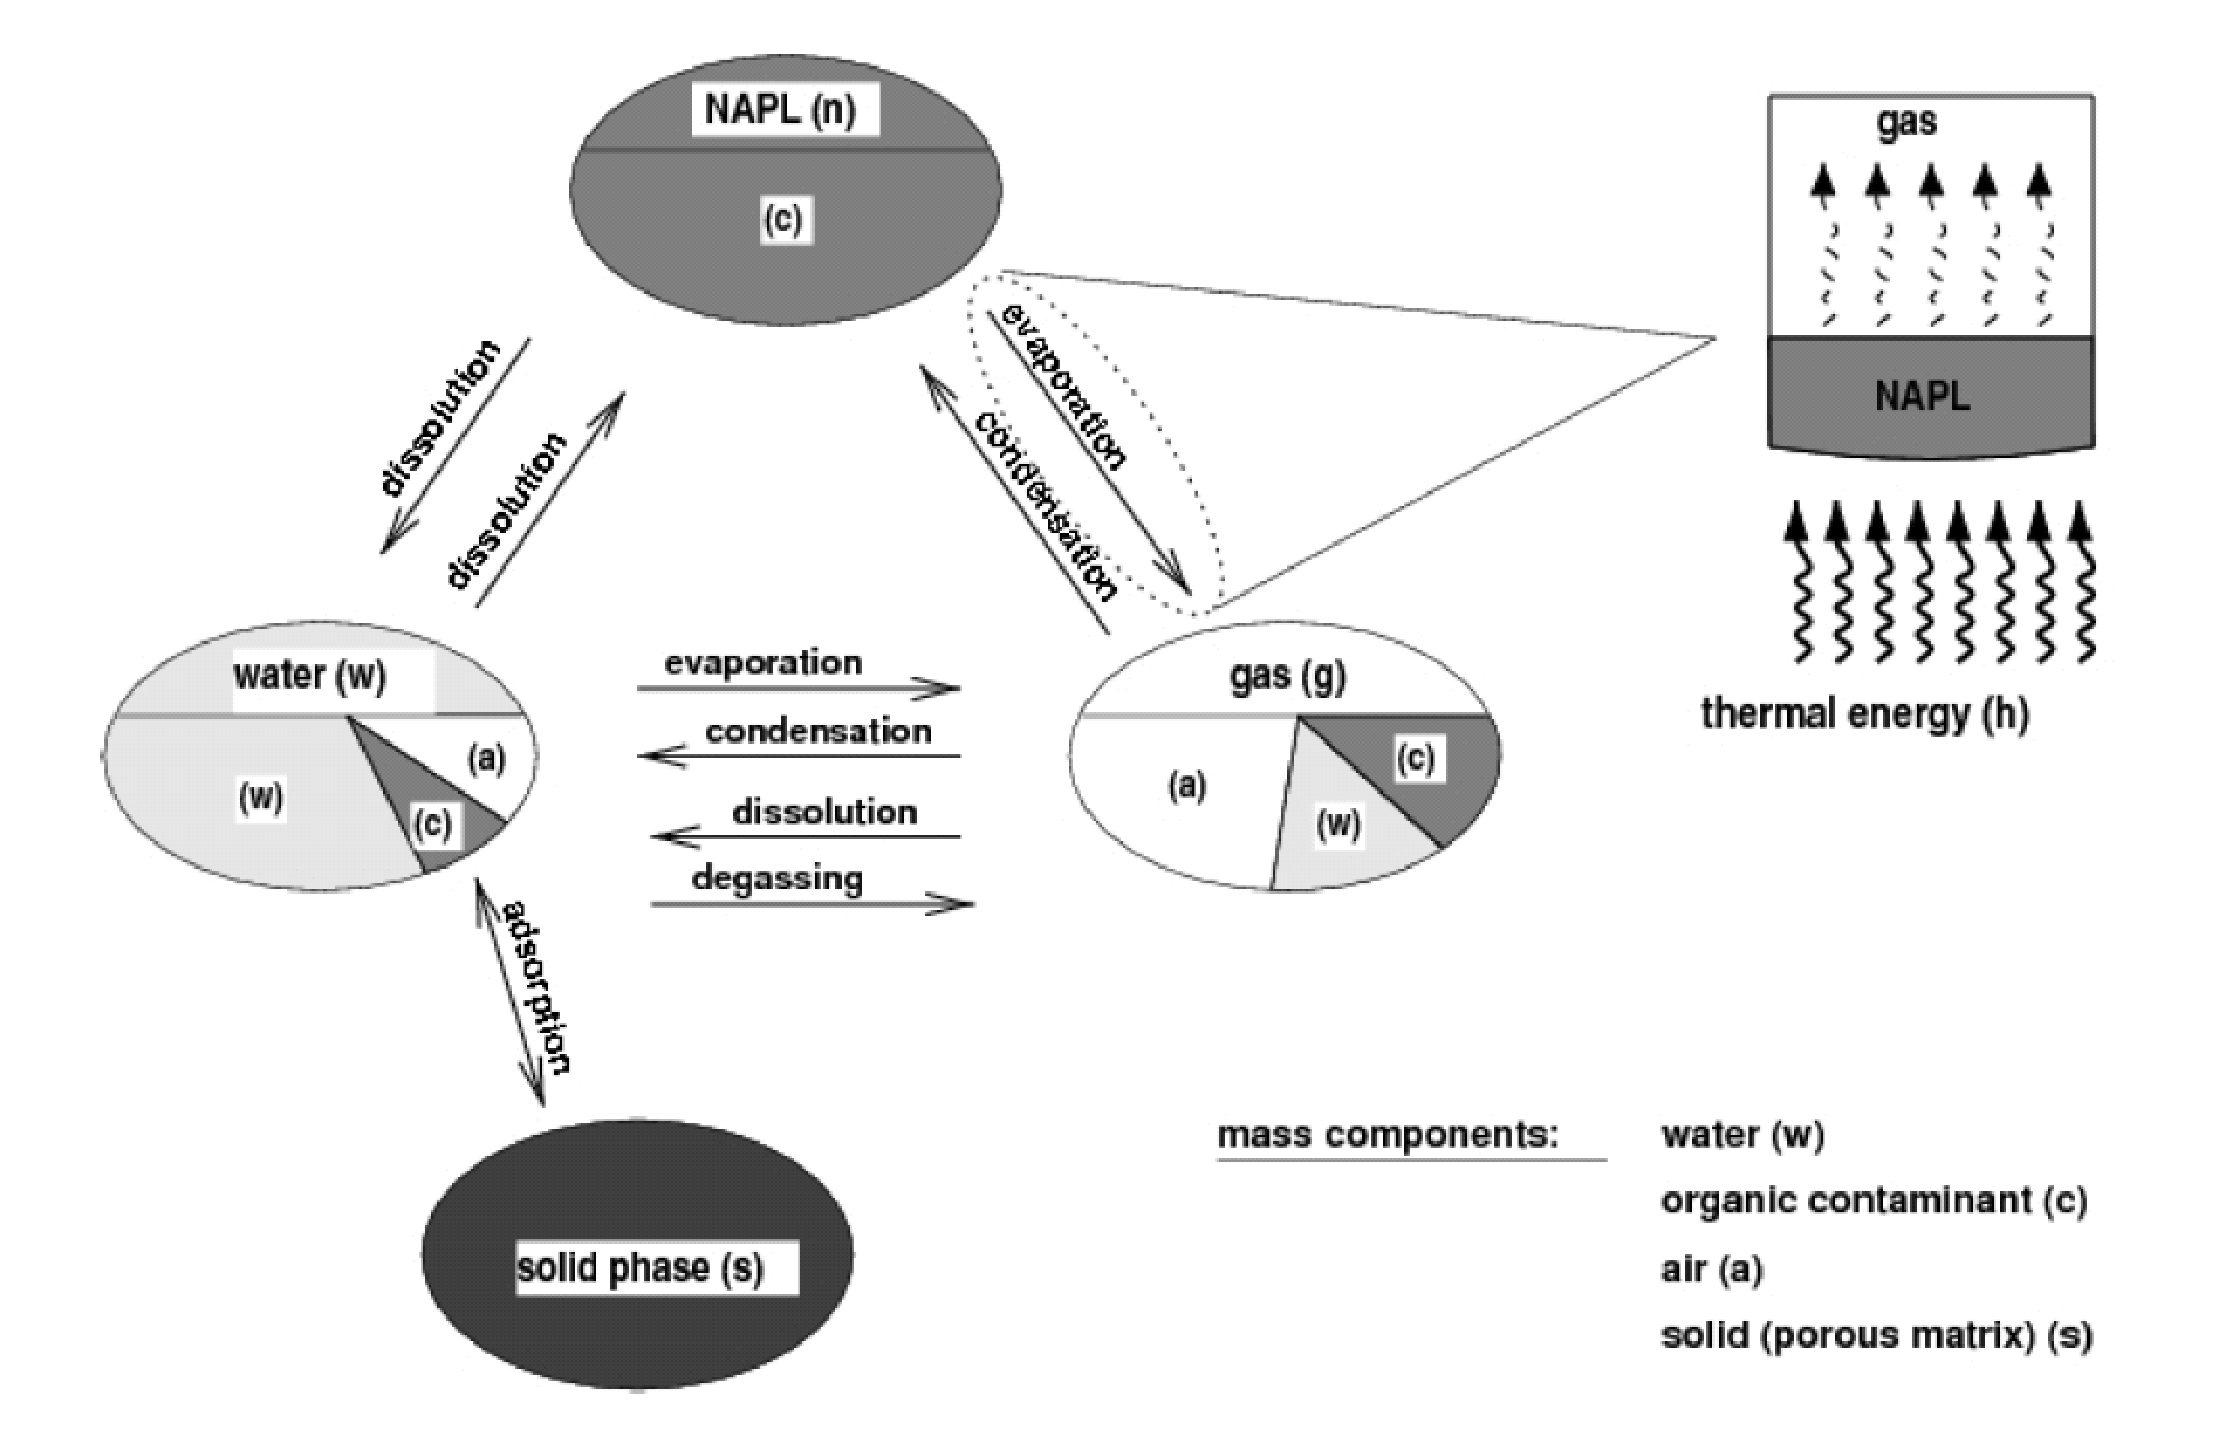
\includegraphics[width=0.7\linewidth]{EPS/masstransfer}
  \caption{Mass and energy transfer between the phases}
  \label{A3:fig:mundwtrans}
\end{figure}

\textbf{Equilibrium:}
For the nonisothermal multiphase processes in porous media under
consideration, we state that the assumption of local thermal
equilibrium is valid since flow velocities are small. We neglect
chemical reactions and biological decomposition and assume chemical
equilibrium.  Mechanical equilibrium is not valid in a porous medium, 
since discontinuities in pressure can occur across a fluid-fluid
interface due to capillary effects.

\textbf{Notation:} The index $\alpha \in \{\text{w}, \text{n}, \text{g}\}$ refers 
to the phase, while the superscript $\kappa \in \{\text{w}, \text{a}, \text{c}\}$ refers 
to the component. \\
\begin{tabular}{llll}
$p_\alpha$ & phase pressure & $\phi$ & porosity \\
$T$ & temperature & $K$ & absolute permeability tensor \\
$S_\alpha$ & phase saturation & $\tau$ & tortuosity \\
$x_\alpha^\kappa$ & mole fraction of component $\kappa$ in phase $\alpha$ & $\boldsymbol{g}$ & gravitational acceleration \\
$X_\alpha^\kappa$ & mass fraction of component $\kappa$ in phase $\alpha$ & $q^\kappa_\alpha$ & volume source term of $\kappa$ in $\alpha$ \\
$\varrho_{\text{mol},\alpha}$ & molar density of phase $\alpha$ & $u_\alpha$ & specific internal energy \\
$\varrho_{\alpha}$ & mass density of phase $\alpha$ & $h_\alpha$ & specific enthalpy \\
$k_{\text{r}\alpha}$ & relative permeability & $c_\text{s}$ & specific heat enthalpy \\
$\mu_\alpha$ & phase viscosity & $\lambda_\text{pm}$ & heat conductivity \\
$D_\alpha^\kappa$ & diffusivity of component $\kappa$ in phase $\alpha$ & $q^h$ & heat source term \\
$v_\alpha$ & Darcy velocity & $v_{a,\alpha}$  & advective velocity
\end{tabular}


\subsection{Balance Equations}
For the balance equations for multicomponent systems, it is in many
cases convenient to use a molar formulation of the continuity
equation. Considering the mass conservation for each component allows
us to drop source/sink terms for describing the mass transfer between
phases. Then, the
molar mass balance can be written as:
%
\begin{eqnarray}
  \label{A3:eqmass1}
  && \phi \frac{\partial (\sum_\alpha \varrho_{\text{mol}, \alpha}
    x_\alpha^\kappa S_\alpha )}{\partial t} \nonumber 
 - \sum\limits_\alpha \Div \left( \frac{k_{\text{r}
        \alpha}}{\mu_\alpha} \varrho_{\text{mol}, \alpha}
    x_\alpha^\kappa K (\grad p_\alpha -
    \varrho_{\alpha} \boldsymbol{g}) \right) \nonumber \\
  %
  \nonumber \\
  %
  && - \sum\limits_\alpha \Div \left( \tau \phi S_\alpha D_\alpha^\kappa \varrho_{\text{mol},
      \alpha} \grad x_\alpha^\kappa \right) \nonumber 
 - q^\kappa = 0, \qquad \kappa \in \{\text{w,a,c}\}.
\end{eqnarray}

The component mass balance can also be written in terms of mass fractions 
by replacing molar densities by mass densities and mole by mass fractions.
To obtain a single conserved quantity in the temporal derivative, the total 
concentration, representing the mass of one component per unit volume, is defined as
\begin{displaymath}
C^\kappa = \sum_\alpha \phi S_\alpha \varrho_{\text{mass},\alpha} X_\alpha^\kappa \; .
\end{displaymath}
Using this definition, the component mass balance is written as:

\begin{eqnarray}
  \label{A3:eqmass2}
  &&  \frac{\partial C^\kappa}{\partial t} = 
  \sum\limits_\alpha \Div \left( \frac{k_{\text{r}
        \alpha}}{\mu_\alpha} \varrho_{\text{mass}, \alpha}
    X_\alpha^\kappa K (\grad p_\alpha +
    \varrho_{\text{mass}, \alpha} \boldsymbol{g}) \right) \nonumber \\
  %
  \nonumber \\
  %
  && + \sum\limits_\alpha \Div \left( \tau \phi S_\alpha D_\alpha^\kappa \varrho_{\text{mass},
      \alpha} \grad X_\alpha^\kappa \right) \nonumber 
 + q^\kappa = 0, \qquad \kappa \in \{\text{w,a,c}\}.
\end{eqnarray}


In the case of non-isothermal systems, we further have to balance the
thermal energy. We assume fully reversible processes, such that entropy
is not needed as a model parameter. Furthermore, we neglect 
dissipative effects and the heat transport due to molecular
diffusion. The heat balance can then be
formulated as:
%
\begin{eqnarray}
  \label{A3:eqenergmak1}
  && \phi \frac{\partial \left( \sum_\alpha \varrho_{\alpha}
      u_\alpha S_\alpha \right)}{\partial t} + \left( 1 -
    \phi \right) \frac{\partial \varrho_{\text{s}} c_{\text{s}}
    T}{\partial t} \nonumber 
 - \Div \left( \lambda_{\text{pm}} \grad T \right)
  \nonumber \\
  %
  \nonumber \\
  %
  && - \sum\limits_\alpha \Div \left( \frac{k_{\text{r}
        \alpha}}{\mu_\alpha} \varrho_{\alpha} h_\alpha
    K \left( \grad p_\alpha - \varrho_{\alpha}
      \boldsymbol{g} \right) \right) \nonumber 
 - q^h \; = \; 0.
\end{eqnarray}

In order to close the system, supplementary constraints for capillary pressure, saturations and mole
fractions are needed, \cite{A3:helmig:1997}. 
According to the Gibbsian phase rule, the number of degrees of freedom
in a non-isothermal compositional multiphase system is equal to the
number of components plus one. This means we need as many independent
unknowns in the system description. The
available primary variables are, e.\ g., saturations, mole/mass
fractions, temperature, pressures, etc.




\section{Available models} 
The following description of the available models is automatically extracted 
from the Doxygen documentation. \textbf{TODO}: Unify notation. 

\subsection{Fully coupled models} 

\subsubsection{The single-phase model: OnePBoxModel} 
%%%%%%%%%%%%%%%%%%%%%%%%%%%%%%%%%%%%%%%%%%%%%%%%%%%%%%%%%%%%%%%%%
% This file has been autogenerated from the LaTeX part of the   %
% doxygen documentation; DO NOT EDIT IT! Change the model's .hh %
% file instead!!                                                %
%%%%%%%%%%%%%%%%%%%%%%%%%%%%%%%%%%%%%%%%%%%%%%%%%%%%%%%%%%%%%%%%%

\-Single-\/phase, isothermal flow model, which solves the mass continuity equation \[ \phi \frac{\partial \varrho}{\partial t} + \text{div} (- \varrho \frac{\textbf K}{\mu} ( \textbf{grad}\, p -\varrho {\textbf g})) = q, \] discretized using a vertex-\/centered finite volume (box) scheme as spatial and the implicit \-Euler method as time discretization. \-The model supports compressible as well as incompressible fluids.



\subsubsection{The single-phase, two-component model:  OnePTwoCBoxModel} 
%%%%%%%%%%%%%%%%%%%%%%%%%%%%%%%%%%%%%%%%%%%%%%%%%%%%%%%%%%%%%%%%%
% This file has been autogenerated from the LaTeX part of the   %
% doxygen documentation; DO NOT EDIT IT! Change the model's .hh %
% file instead!!                                                %
%%%%%%%%%%%%%%%%%%%%%%%%%%%%%%%%%%%%%%%%%%%%%%%%%%%%%%%%%%%%%%%%%

\-This model implements a one-\/phase flow of a compressible fluid, that consists of two components, using a standard \-Darcy approach as the equation for the conservation of momentum\-: \[ v_{D} = - \frac{\textbf K}{\mu} \left(\text{grad} p - \varrho {\textbf g} \right) \]

\-Gravity can be enabled or disabled via the property system. \-By inserting this into the continuity equation, one gets \[ \Phi \frac{\partial \varrho}{\partial t} - \text{div} \left\{ \varrho \frac{\textbf K}{\mu} \left(\text{grad}\, p - \varrho {\textbf g} \right) \right\} = q \;, \]

\-The transport of the components is described by the following equation\-: \[ \Phi \frac{ \partial \varrho x}{\partial t} - \text{div} \left( \varrho \frac{{\textbf K} x}{\mu} \left( \text{grad}\, p - \varrho {\textbf g} \right) + \varrho \tau \Phi D \text{grad} x \right) = q. \]

\-All equations are discretized using a fully-\/coupled vertex-\/centered finite volume (box) scheme as spatial and the implicit \-Euler method as time discretization.

\-The primary variables are the pressure $p$ and the mole or mass fraction of dissolved component $x$.



\subsubsection{The two-phase model using Richards' assumption: RichardsBoxModel} 
Here comes the detailed documentation. 


\subsubsection{The two-phase model: TwoPBoxModel}
You can pick the formulation by setting the \char`\"{}Formulation\char`\"{} property. The default is pW-Sn. 


\subsubsection{The non-isothermal two-phase model: TwoPNIBoxModel} 
%%%%%%%%%%%%%%%%%%%%%%%%%%%%%%%%%%%%%%%%%%%%%%%%%%%%%%%%%%%%%%%%%
% This file has been autogenerated from the LaTeX part of the   %
% doxygen documentation; DO NOT EDIT IT! Change the model's .hh %
% file instead!!                                                %
%%%%%%%%%%%%%%%%%%%%%%%%%%%%%%%%%%%%%%%%%%%%%%%%%%%%%%%%%%%%%%%%%

\-This model implements a non-\/isothermal two-\/phase flow for two immiscible fluids $\alpha \in \{ w, n \}$. \-Using the standard multiphase \-Darcy approach, the mass conservation equations for both phases can be described as follows\-: \[ \phi \frac{\partial \phi \varrho_\alpha S_\alpha}{\partial t} - \text{div} \left\{ \varrho_\alpha \frac{k_{r\alpha}}{\mu_\alpha} \mathrm{K} \left( \textrm{grad}\, p_\alpha - \varrho_{\alpha} \mathbf{g} \right) \right\} - q_\alpha = 0 \qquad \alpha \in \{w, n\} \]

\-For the energy balance, local thermal equilibrium is assumed. \-This results in one energy conservation equation for the porous solid matrix and the fluids\-:

\begin{align*} \frac{\partial \phi \sum_alpha \varrho_\alpha u_\alpha S_\alpha}{\partial t} & + \left( 1 - \phi \right) \frac{\partial (\varrho_s c_s T)}{\partial t} - \sum_\alpha \text{div} \left\{ \varrho_\alpha h_\alpha \frac{k_{r\alpha}}{\mu_\alpha} \mathbf{K} \left( \textbf{grad}\,p_\alpha - \varrho_\alpha \mbox{\bf g} \right) \right\} \\ & - \text{div} \left(\lambda_{pm} \textbf{grad} \, T \right) - q^h = 0, \qquad \alpha \in \{w, n\} \;, \end{align*} where $h_\alpha$ is the specific enthalpy of a fluid phase $\alpha$ and $u_\alpha = h_\alpha - p_\alpha/\varrho_\alpha$ is the specific internal energy of the phase.

\-The equations are discretized using a fully-\/coupled vertex centered finite volume (box) scheme as spatial and the implicit \-Euler method as time discretization.

\-Currently the model supports choosing either $p_w$, $S_n$ and $T$ or $p_n$, $S_w$ and $T$ as primary variables. \-The formulation which ought to be used can be specified by setting the {\ttfamily \-Formulation} property to either {\ttfamily \-Two\-P\-N\-I\-Indices\-::p\-Ws\-N} or {\ttfamily \-Two\-P\-Indices\-::p\-Ns\-W}. \-By default, the model uses $p_w$, $S_n$ and $T$.



\subsubsection{The two-phase, two-component model: TwoPTwoCBoxModel} 
%%%%%%%%%%%%%%%%%%%%%%%%%%%%%%%%%%%%%%%%%%%%%%%%%%%%%%%%%%%%%%%%%
% This file has been autogenerated from the LaTeX part of the   %
% doxygen documentation; DO NOT EDIT IT! Change the model's .hh %
% file instead!!                                                %
%%%%%%%%%%%%%%%%%%%%%%%%%%%%%%%%%%%%%%%%%%%%%%%%%%%%%%%%%%%%%%%%%


Adaption of the BOX scheme to the two-\/phase two-\/component flow model. This model implements two-\/phase two-\/component flow of two compressible and partially miscible fluids $\alpha \in \{ w, n \}$ composed of the two components $\kappa \in \{ w, a \}$. The standard multiphase Darcy approach is used as the equation for the conservation of momentum: \[ v_\alpha = - \frac{k_{r\alpha}}{\mu_\alpha} \mbox{\bf K} \left(\text{grad}\, p_\alpha - \varrho_{\alpha} \mbox{\bf g} \right) \]

By inserting this into the equations for the conservation of the components, one gets one transport equation for each component \begin{eqnarray} && \phi \frac{\partial (\sum_\alpha \varrho_\alpha X_\alpha^\kappa S_\alpha )} {\partial t} - \sum_\alpha \text{div} \left\{ \varrho_\alpha X_\alpha^\kappa \frac{k_{r\alpha}}{\mu_\alpha} \mbox{\bf K} (\text{grad}\, p_\alpha - \varrho_{\alpha} \mbox{\bf g}) \right\} \nonumber \\ \nonumber \\ &-& \sum_\alpha \text{div} \left\{{\bf D_{\alpha, pm}^\kappa} \varrho_{\alpha} \text{grad}\, X^\kappa_{\alpha} \right\} - \sum_\alpha q_\alpha^\kappa = 0 \qquad \kappa \in \{w, a\} \, , \alpha \in \{w, g\} \end{eqnarray}

This is discretized using a fully-\/coupled vertex centered finite volume (box) scheme as spatial and the implicit Euler method as temporal discretization.

By using constitutive relations for the capillary pressure $p_c = p_n - p_w$ and relative permeability $k_{r\alpha}$ and taking advantage of the fact that $S_w + S_n = 1$ and $X^\kappa_w + X^\kappa_n = 1$, the number of unknowns can be reduced to two. The used primary variables are, like in the two-\/phase model, either $p_w$ and $S_n$ or $p_n$ and $S_w$. The formulation which ought to be used can be specified by setting the {\ttfamily Formulation} property to either TwoPTwoCIndices::pWsN or TwoPTwoCIndices::pNsW. By default, the model uses $p_w$ and $S_n$. Moreover, the second primary variable depends on the phase state, since a primary variable switch is included. The phase state is stored for all nodes of the system. Following cases can be distinguished:
\begin{itemize}
\item Both phases are present: The saturation is used (either $S_n$ or $S_w$, dependent on the chosen {\ttfamily Formulation}), as long as $ 0 < S_\alpha < 1$.
\item Only wetting phase is present: The mass fraction of, e.g., air in the wetting phase $X^a_w$ is used, as long as the maximum mass fraction is not exceeded ( $X^a_w<X^a_{w,max}$)
\item Only non-\/wetting phase is present: The mass fraction of, e.g., water in the non-\/wetting phase, $X^w_n$, is used, as long as the maximum mass fraction is not exceeded ( $X^w_n<X^w_{n,max}$)
\end{itemize}



\subsubsection{The non-isothermal two-phase, two-component model: TwoPTwoCNIBoxModel} 
This implements a non-isothermal two-phase two-component model with Pw and Sn/X as primary unknowns. You can use Pn and Sw/X as primary variables if you set the Formulation property to pNsW. 



\subsection{Decoupled models}

\subsubsection{FractionalFlow Model}
The model implements the decoupled equations of two-phase flow of two completely immiscible fluids. These equations can be derived from the two-phase flow equations shown for the two-phase box model (\doxyref{TwoPBoxModel}{p.}{classDune_1_1TwoPBoxModel}). The first equation to solve is a pressure equation of elliptic character. The second one is a saturation equation, which can be hyperbolic or parabolic.

This model allows different combinations of primary variables, which can be $p_w$-$S_w$, $p_w$-$S_n$, $p_n$-$S_w$, $p_n$-$S_n$, or $p$-$S_w$ and $p$-$S_n$, where $p$ is no phase pressure but a global pressure.

As the equations are only weakly coupled they do not have to be solved simultaneously but can be solved sequentially. First the pressure equation is solved implicitly, second the saturation equation can be solved explicitly. This solution procedure is called \doxyref{IMPES}{p.}{classDune_1_1IMPES} algorithm (IMplicit Pressure Explicit Saturation).

In comparison to a fully coupled model, different discretization methods can be applied to the different equations. So far, the pressure equation is discretized using a cell centered finite volume scheme (optionally with multi point flux approximation), a mimetic finite difference scheme or a finite element scheme. The saturation equation is discretized using a cell centered finite volume scheme. Default time discretization scheme is an explicit Euler scheme. 

\subsubsection{Decoupled2p2c}

(Extracted from decoupled2p2c.hh:) 
Implementation of a decoupled formulation of a two phase two component flow processin porous media.

This implementation is written for a liquid-gas system. For the physical description of gas and liquid derivations of the classes \doxyref{Gas\_\-GL}{p.}{classDune_1_1Gas__GL} and \doxyref{Liquid\_\-GL}{p.}{classDune_1_1Liquid__GL} have to be provided. The template parameters are the used grid class and the desired number type (usually double) The pressure equation is given as $ -\frac{\partial V}{\partial p}\frac{\partial p}{\partial t}+\sum_{\kappa}\frac{\partial V}{\partial m^{\kappa}}\nabla\cdot\left(\sum_{\alpha}C_{\alpha}^{\kappa}\mathbf{v}_{\alpha}\right)=\sum_{\kappa}\frac{\partial V}{\partial m^{\kappa}}q^{\kappa}$ See paper SPE 99619 for derivation. The transport equation is $ \frac{\partial C^\kappa}{\partial t} = - \nabla \cdot \sum{C_\alpha^\kappa f_\alpha {\bf v}} + q^\kappa $

The pressure equation is given as $ -\frac{\partial V}{\partial p}\frac{\partial p}{\partial t}+\sum_{\kappa}\frac{\partial V}{\partial m^{\kappa}}\nabla\cdot\left(\sum_{\alpha}C_{\alpha}^{\kappa}\mathbf{v}_{\alpha}\right)=\sum_{\kappa}\frac{\partial V}{\partial m^{\kappa}}q^{\kappa}$ See paper SPE 99619 for derivation. The transport equation is $ \frac{\partial C^\kappa}{\partial t} = - \nabla \cdot \sum{C_\alpha^\kappa f_\alpha {\bf v}} + q^\kappa $ 






%%% Local Variables: 
%%% mode: latex
%%% TeX-master: "dumux-handbook"
%%% End: 
